\documentclass[11pt]{article}

\usepackage[margin=1.05in]{geometry}
\usepackage{amsmath,amssymb,amsthm}
\usepackage{graphicx}
\usepackage{enumitem}
\usepackage[round]{natbib}
\usepackage{microtype}

\graphicspath{{figures/}}
\setlength{\parindent}{0em}
\setlength{\parskip}{0.4em}
\setlength{\emergencystretch}{3em}

\newtheorem{proposition}{Proposition}
\newcommand{\dd}{\mathrm d}
\newcommand{\E}{\mathbb E}

\title{Intergenerational Housing Misallocation and Fertility\\[-0.1em]
\large Short model note}
\author{Tommaso De Santo}
\date{June 2026}

\begin{document}
\maketitle


\section{Environment}

The economy is populated by overlapping generations of young and old households. A young household has type $i=(y_i,a_i,B_i)$: income, liquid wealth, and the gross bequest assigned at entry, taxed on receipt. She decides whether to enter the housing market; inside, she chooses a tenure, a house size, completed fertility, and savings for old age. Old households, indexed by $j$ as young households are by $i$, are of two kinds: old incumbents, last period's young owners, who enter old age with financial wealth, the house they bought, and a possible accrued gain, choose how much of the house to keep and how large an estate to leave, then exit; and old renters, last period's young renter entrants, who rent in old age and carry no wedge. Nonentrants stay outside the market in both periods. Each period a mass $\bar M$ of potential young households enters the pool: the maturing children of the previous cohort plus a renewal inflow. Types are distributed according to $G_Y$, and newborns inherit the estates of the old who exit as they arrive.

\textbf{Preferences.} Households have preferences over consumption, housing, and children. Children raise the household's consumption and housing needs: each child claims $\chi>0$ units of consumption and $\kappa>0$ units of space, so with consumption spending $c_i$, housing $h_i$, and fertility $n_i$,
\[
u_i^Y=\log(c_i-\chi n_i)+\alpha\log(h_i-\kappa n_i)+\vartheta\log n_i .
\]
Rearranging a budget at user cost $q$ shows what a child costs,
\[
(c_i-\chi n_i)+q\,(h_i-\kappa n_i)+(\chi+\kappa q)\,n_i=c_i+q h_i :
\]
its consumption requirement plus the market value of the space it occupies. A useful benchmark is equal scaling, $\chi=\kappa q/\alpha$, under which a child uses consumption and space in the same proportions as its parents. Old households value consumption, housing, and the estate $e_j\ge0$ they leave at exit:
\[
u^O=\log c_j^O+\gamma\log h_j^O+\mathcal B(e_j),
\]
with $\mathcal B$ a warm-glow function, increasing and concave, possibly zero, common to all old households. The exiting cohort's estates are what the arriving cohort inherits as the $B_{i'}$. A young household also values her own old age: her objective adds $\beta\,u^O$, evaluated at the old-age choices she will make, with discount factor $\beta\in(0,1]$.

\textbf{Housing.} There is a fixed stock $\bar H$ of divisible floorspace. Renting and owning are occupancy modes with different size menus,
\[
h\le\bar h^R \text{ (rent)},
\qquad
h\le\bar h^O \text{ (own)},
\qquad
\bar h^R<\bar h^O ,
\]
Family-sized houses are mostly available to buy, not to rent. All floorspace trades in one market: the asset price is $P$, and no-arbitrage ties the rental rate to it,
\[
q=\rho P,
\qquad
\rho=r+\delta+\tau^p .
\]
Given $q$, a higher property tax lowers $P$ and with it the down payment on any given house. Lowercase $h$ is an occupancy choice; capital $H$ marks housing quantities not chosen today: the stock, the caps, carried housing.

\textbf{Financing.} A buyer finances at most a share $\phi\in(0,1)$ of the purchase, so the down payment is $(1-\phi)Ph$, posted at purchase from wealth in hand, $A_i(x)=a_i+xB_i+T_i^b(x)$ with $x=1-\tau^b$, where $\tau^b$ is the estate tax, $T_i^b(x)$ the estate-tax rebate assigned to type $i$, and $B_i$ the assigned bequest; housing payments may not exceed $\psi y_i$, with $\psi\in(0,1)$. The down payment is capped by wealth because income arrives only over the period. Wealth is otherwise fungible: it enters the budget alongside income, and buying assets is not expenditure, so the posted equity remains the household's. Households save: a young household carries $a_i'\ge0$ into old age at the exogenous gross return $1+r$, with no unsecured borrowing against old age; a renter, with no asset to pledge, therefore cannot borrow at all. The interest rate $r$ is exogenous: households borrow and lend with a passive financial sector, so the only price determined inside the model is $q$.

\textbf{Capital-gains taxation.} A sale during life realizes the seller's accrued gain, taxed at rate $\tau^g$ above an exclusion. A house held until death passes with a stepped-up basis, and the gain is never taxed. Where the gains come from is a modeling device, stated plainly: the model is real, the tax code computes gains in dollars, and steady inflation $\varpi$ with constant relative prices gives every cohort's unit the same nominal gain. Selling triggers the real tax $\bar\ell=\tau^g P\varpi/(1+\varpi)$ per unit, zero below the exclusion; inflation enters the model nowhere else. So $\ell_j=\bar\ell$ for an old incumbent whose gain clears the exclusion---larger holdings clear the level exclusion---and the gain is deterministic: a buyer knows the tax her future self will face.

\section{Households}

Conditional on entry, household $i$ chooses a tenure mode $m\in\{R,O\}$, a bundle, and savings. The two modes share one objective and one budget; they differ in the size menu and in whether the financing constraints apply. For $m\in\{R,O\}$,
\[
\begin{aligned}
W_i^m=\max_{c_i,h_i,n_i,a_i'}\;&
\log(c_i-\chi n_i)+\alpha\log(h_i-\kappa n_i)+\vartheta\log n_i\\
&+\beta\big[\mathbf 1\{m=R\}\,V^R(a_{j'})+\mathbf 1\{m=O\}\,V^O(a_{j'},h_i,\ell_{i'})\big]
\end{aligned}
\]
subject to
\[
c_i+q h_i+a_i'=y_i+A_i(x),
\qquad
h_i\le\bar h^m,
\qquad
a_i'\ge0,
\]
\[
\mathbf 1\{m=O\}\,(1-\phi)P h_i\le A_i(x),
\qquad
\mathbf 1\{m=O\}\,q h_i\le\psi y_i .
\]
The old state is generated by the household's own choices: financial wealth $a_{j'}=(1+r)\,a_i'-\mathbf 1\{m=O\}\,q h_i$---real wealth is conserved, the nominal gain is not wealth---and the tax state $\ell_{i'}=\bar\ell$ if $h_i$ clears the exclusion, zero below. Nothing is random; $V^O$ and $V^R$ are the old values defined next.

The old incumbent enters with financial wealth $a_j$, housing $H_j^0$, and the tax state $\ell_j$. Each unit she holds faces one choice: sell now and pay the tax, or keep it until death, when the tax is forgiven. She solves
\[
\begin{aligned}
V^O(a_j,H_j^0,\ell_j)
&=\max_{c_j^O,\,h_j^O,\,e_j}\;u^O(c_j^O,h_j^O,e_j)
\\
&\text{subject to}\quad
c_j^O+e_j+q\,h_j^O=a_j+qH_j^0-\ell_j\,(H_j^0-h_j^O),
\qquad
0\le h_j^O\le H_j^0 .
\end{aligned}
\]
Selling a unit nets $q-\ell_j$; the forgiveness at death is a subsidy to staying put, a transfer rather than a resource saving. An old renter has no carried housing and no tax:
\[
V^R(a_j)
=\max_{c_j^O,\,h_j^O,\,e_j}\;u^O(c_j^O,h_j^O,e_j)
\quad\text{subject to}\quad
c_j^O+e_j+q\,h_j^O=a_j,
\qquad
0<h_j^O\le\bar h^R ,
\]
and at an interior choice her marginal value of space is exactly $q$.

Individuals save, and savings are the old's resources. They are pinned by the Euler equation
\[
\frac{1}{c_i-\chi n_i}=\beta(1+r)\,\frac{1}{c_{j'}^O}
\qquad\text{when }a_i'>0,
\]
which under logarithmic old utility (warm glow $b\log e$ included) and interior old choices collapses to a savings rule:
\[
a_i'=k\,(c_i-\chi n_i)+\frac{\ell_{i'}\,h_i}{1+r},
\qquad
k=\beta\left(1+\gamma+b\right):
\]
the household saves old age's claim on adult consumption plus her discounted future tax bill, so anticipating the lock-in tax is itself a savings motive. By the same conversion, a buyer above the exclusion pays an effective price $q^O=q+\bar\ell/(1+r)$ per unit of space---the market price plus her own discounted lock-in tax---while a renter or a below-exclusion buyer pays $q$. A unit of adult consumption commits $1+k$ units of resources, one spent now and $k$ carried.

When no cap binds, the problem solves in one line: with lifetime resources $w_i=y_i+A_i(x)$ and the branch's effective price $q^m$,
\[
c_i-\chi n_i=\frac{w_i}{1+\alpha+\vartheta+k},
\qquad
n_i=\frac{\vartheta\,w_i}{(1+\alpha+\vartheta+k)(\chi+\kappa q^m)},
\qquad
h_i=\frac{\alpha\,w_i}{(1+\alpha+\vartheta+k)\,q^m}+\kappa n_i,
\]
and savings follow the rule above. When the cap binds, $h_i=H_i^m$, fertility solves the condition displayed in the last section, and the budget gives the rest.

Using $P=q/\rho$, owner housing is bounded by
\[
H_i^O=\min\left\{\bar h^O,\;\frac{A_i(x)\,\rho}{(1-\phi)\,q},\;\frac{\psi y_i}{q}\right\},
\qquad
H_i^R=\bar h^R .
\]
$H_i^m$ is the effective family-housing cap: a renter is capped by the stock, a buyer by whichever of menu, collateral, or debt service is shortest. Tenure is $W_i^Y=\max\{W_i^R,W_i^O\}$. Entry compares the inside value with an outside option $\bar W^E$ under extreme-value shocks of scale $\kappa_E$:
\[
\pi_i^E=\frac{\exp\{W_i^Y/\kappa_E\}}{\exp\{W_i^Y/\kappa_E\}+\exp\{\bar W^E/\kappa_E\}}
\]
is the probability that household $i$ enters.

\section{Equilibrium}

Aggregate demand adds young households, old incumbents, and old renters, and the single market clears:
\[
\bar M\int\pi_i^E\,h_i\,\dd G_Y(i)+\int h_j^O\,\dd F_O(j)+\int h_j^O\,\dd F_R(j)=\bar H ,
\]
where $F_O$ and $F_R$ are the measures of old incumbents and old renters.
A stationary equilibrium is a user cost $q$ (and $P=q/\rho$) such that households optimize, the market clears, fiscal and credit accounts close with lump-sum transfers, next period's old households are this period's young entrants, owners as incumbents and renters as old renters, and births plus the renewal inflow keep the cohort at $\bar M$. Nothing in the clearing condition asks whether the marginal family-sized unit is held by the household that values it most; that is the next section's question.

\section{Marginal conditions}

How much a constraint binds can be read off the household's own bundle. The branch problem's Lagrangian is
\[
\begin{aligned}
\mathcal L=\;&u_i^Y+\beta\,V_{j'}+\lambda_i\big(y_i+A_i(x)-c_i-qh_i-a_i'\big)\\
&+\mu_i\big(A_i(x)-(1-\phi)Ph_i\big)+\eta_i\big(\psi y_i-qh_i\big)+\theta_i\big(\bar h^m-h_i\big),
\end{aligned}
\]
with $\mu_i=\eta_i=0$ in the rental mode and the savings bound $a_i'\ge0$ carried by the Euler complementarity; every condition below is a derivative of $\mathcal L$. At an interior choice, a household's marginal value of space is $u_h/u_c=\alpha(c-\chi n)/(h-\kappa n)$. For a renter,
\[
\frac{\alpha\,(c_i^R-\chi n_i^R)}{h_i^R-\kappa n_i^R}=q+\zeta_i^R,
\]
so $\zeta_i^R\ge0$ measures the bite of the rental menu in goods, computable from the bundle. For a young owner the same gap collects the three access constraints,
\[
\zeta_i^O=\underbrace{\tfrac{\mu_i}{\lambda_i}(1-\phi)P+\tfrac{\eta_i}{\lambda_i}q}_{\zeta_i^{O,F}\text{, financing}}+\underbrace{\tfrac{\theta_i}{\lambda_i}}_{\text{menu}},
\qquad
\frac{\alpha\,(c_i^O-\chi n_i^O)}{h_i^O-\kappa n_i^O}=q^O+\zeta_i^O ,
\]
where $\lambda_i$ is the marginal utility of resources; when the owner menu is slack, the bundle identifies the financing part alone, $\zeta_i^{O,F}=\alpha(c_i^O-\chi n_i^O)/(h_i^O-\kappa n_i^O)-q^O$, the gap over market rent net of the known tax wedge. For an old incumbent at an interior retention choice,
\[
\frac{\gamma c_j^O}{h_j^O}=q-\ell_j :
\]
she keeps marginal space she values below what the market would pay, because selling it would realize the taxable gain. Old renters carry no such wedge: their marginal value is $q$.

The gaps price children. Multiplying the fertility first-order condition by consumption gives, in either tenure,
\[
\frac{\vartheta\,(c_i^m-\chi n_i^m)}{n_i^m}=\chi+\kappa\,(q^m+\zeta_i^m),
\]
with $q^m$ the branch's effective price.
A child's space requirement is priced at the household's own shadow value of space. Children get more expensive exactly where family-sized space is hard to reach, with market prices unchanged.

\section{Efficiency}

The planner faces the economy's real constraints and nothing else: the stock, the size menus, goods feasibility, and the domain conditions. It does not face household budgets, since allocations are supported by lump-sum transfers, and it does not face the financing inequalities, which restrict market purchases rather than occupancy. Let $r_i^F\ge0$ be the marginal real cost of implementing one more unit of owner space for a financing-constrained household: zero if the planner can reassign directly, positive if it must work through costly instruments, infinite if the constraint is a primitive nothing relaxes.

\begin{proposition}
Hold the stationary cross-section, entry, tenure assignments, and savings fixed. The planner's surplus from moving one unit of space from an old incumbent at an interior retention choice to a young owner whose owner menu is slack and whose financing constraints bind is
\[
\left(q^O+\zeta_i^{O,F}-r_i^F\right)-\left(q-\ell_j\right)=\zeta_i^{O,F}+\frac{\ell_{i'}}{1+r}+\ell_j-r_i^F .
\]
The competitive allocation solves the planner's conditional problem only if no feasible pair has positive surplus. Conversely, if all financing gaps and levies are zero, the allocation satisfies the planner's conditional first-order conditions.
\end{proposition}

The proof is one variation: move $\dd h$ between the two households, hold each at its prior utility with lump-sum transfers, and the residual $(\zeta_i^{O,F}+\ell_{i'}/(1+r)+\ell_j-r_i^F)\,\dd h$ in goods is left over, a Pareto improvement under any welfare weights; both tax terms are transfers the planner recovers. Two cautions. Real menus are not market failures: a planner facing the same stock is pinned with the renter at $\bar h^R$. And a positive financing gap is an inefficiency only when an instrument can reach it at real cost below the value gap.

\textbf{The two margins in one picture.} Figure~\ref{fig:example} draws a solved stationary case as theory. On the left, the buyer's marginal value of space falls along her constrained path and sits above her effective price by the financing gap $\zeta^{O,F}$ at her cap, while the incumbent's sits below the market price by her tax $\ell$; moving one unit between them frees $\zeta^{O,F}+\bar\ell/(1+r)+\ell$ in goods. On the right, completed fertility rises with the cap at rate $\dd n/\dd H$ until the cap stops binding at $h^u$. The numbers behind the curves are in the long version.

\begin{figure}[t]
\centering
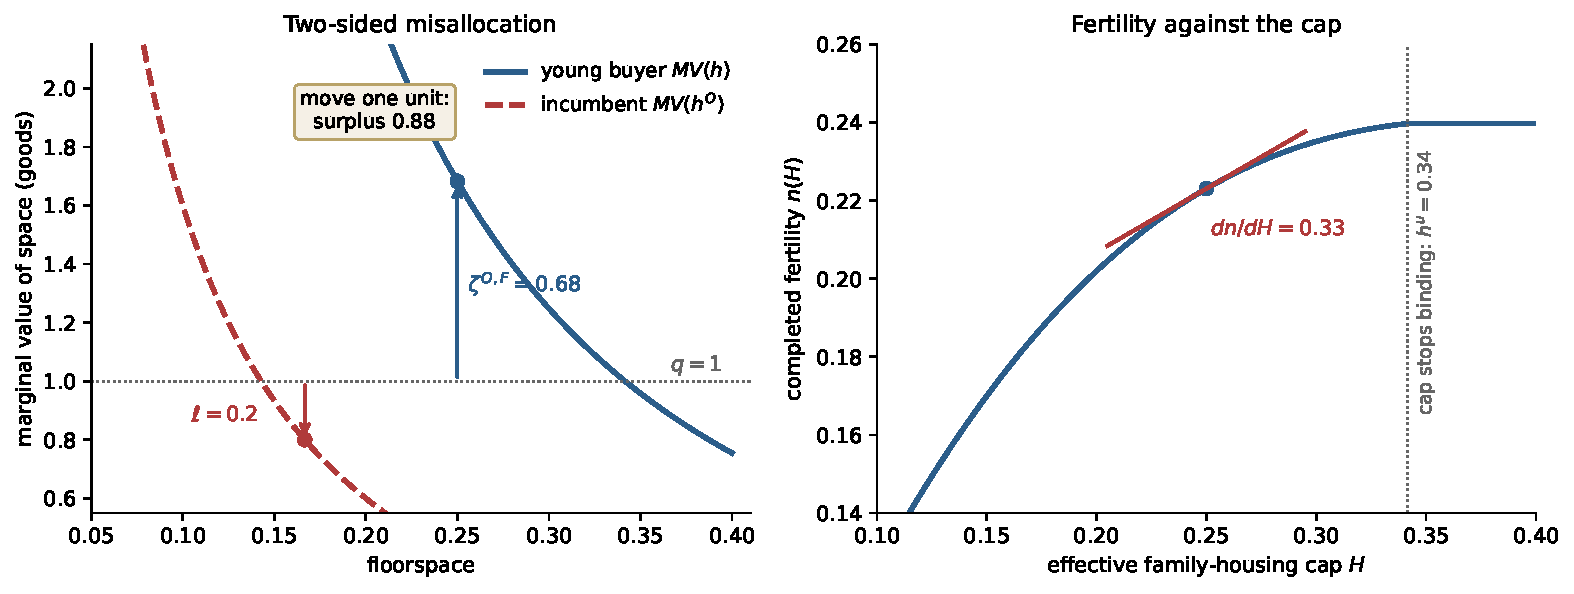
\includegraphics[width=0.96\textwidth]{example_misallocation.pdf}
\caption{Two-sided misallocation and the fertility margin. Left: the collateral-capped buyer values marginal space at $q^O+\zeta^{O,F}$, above the market price; the locked-in incumbent values it at $q-\ell$, below; the distance between the two points is the recoverable surplus. Right: completed fertility against the effective family-housing cap, with slope $\dd n/\dd H$ at the equilibrium cap; the cap stops binding at $h^u$.}
\label{fig:example}
\end{figure}

\section{Fertility and policy}

Fix a tenure branch, let $H$ be the effective cap, write $w=y+A(x)$ for lifetime resources, and let $q^m$ be the branch's effective price. Concentrating the savings rule into the budget, a binding cap makes fertility solve $\vartheta/n=(1+k)\chi/(w-q^mH-\chi n)+\alpha\kappa/(H-\kappa n)$, and
\[
\frac{\dd n}{\dd H}
=
\frac{\dfrac{\alpha\kappa}{(H-\kappa n)^2}-\dfrac{(1+k)\,\chi q^m}{(w-q^mH-\chi n)^2}}
{\dfrac{\vartheta}{n^2}+\dfrac{(1+k)\,\chi^2}{(w-q^mH-\chi n)^2}+\dfrac{\alpha\kappa^2}{(H-\kappa n)^2}} ,
\]
which is positive for every binding cap if and only if $\chi\le(1+k)\,\kappa q^m/\alpha$: relaxing access raises fertility whenever the child's consumption requirement does not exceed its space requirement priced at the lifetime cost of adult consumption. The savings margin loosens the condition because forced housing spending now crowds out saving alongside consumption.

At fixed prices, a small policy $z$ moves aggregate fertility through the constrained:
\[
\left.\frac{\dd N}{\dd z}\right|_{q}
=
\bar M\sum_{m}\int_{\mathcal E_m(z)}
\left[\pi_i^E\,\Psi_i^m+n_i^m\,\frac{\pi_i^E(1-\pi_i^E)}{\kappa_E}\,\Theta_i^m\right]
\mathcal P_i^m(z)\,\dd G_Y(i),
\]
where $\mathcal E_m(z)$ is the set of households whose cap binds in branch $m$, $\mathcal P_i^m=\partial H_i^m/\partial z$ is the pass-through of the policy to the binding component of the cap, $\Psi_i^m=\dd n/\dd H$ is the fertility response, and $\Theta_i^m=\zeta_i^m/(c_i^m-\chi n_i^m)$ drives the entry term. A policy aimed at a slack constraint moves nothing: a down-payment grant does nothing for a household pinned by the rental menu. A transfer of spendable resources also moves fertility through the budget at a fixed cap; the formula isolates the access channel. At $\chi=(1+k)\kappa q^m/\alpha$, equal scaling at lifetime prices, $\Psi_i^m$ is proportional to $\zeta_i^m/(c_i^m-\chi n_i^m)$, so the same gap that measures misallocation predicts whose fertility responds.

Because tenure is a discrete choice, a policy that shifts $W_i^O-W_i^R$ also moves households across the tenure boundary. Below the exclusion both tenures price space at the same $q$, an indifferent household has the same allocation in both, and the switching jump is exactly zero. Above it, the anticipated tax makes owning the dear way to occupy space, and it also hands the owner branch a constant old-age subsidy---occupying retained space at $q-\bar\ell$---that shifts who sits at the boundary without moving any bundle. The long version prices the tension: the switcher into ownership upsizes when the wedge dominates the subsidy in resources, and she has more children when the space force dominates the subsidy's level shift; at the example's parameters both hold with room, and the boundary household upsizes from $0.15$ to $0.20$ and adds $0.007$ children. The long version of the note states and proves this, together with the stationary demographic closure and the full equilibrium definition.

\end{document}
